\documentclass{article}

\usepackage{amssymb}
\usepackage{amsfonts}
\usepackage[tbtags]{amsmath}
\usepackage{amscd}
\usepackage{amsthm}			% Продвинутая математика
\usepackage{mathtext}
\usepackage{cmap}
\usepackage[T2A]{fontenc}
\usepackage[utf8]{inputenc}			% cp1251
\usepackage[english, russian]{babel}
%\usepackage{literat}
\usepackage{pifont}
\usepackage{bm}
\usepackage{array}			% Ширина столбиков в массиве
\usepackage{dcolumn}
\usepackage{hhline}
\usepackage{multirow}
\usepackage{graphicx}
\usepackage{rotating}
\usepackage{calc}
\usepackage{tabularx}
\usepackage{afterpage}
\usepackage{ifthen}
\usepackage{caption2}
\usepackage{substr}
\usepackage[mathscr]{eucal}  %% My addition
\usepackage{mathrsfs}        %% My addition
\usepackage{hypbmsec}        %% My addition
\usepackage{latexsym}        %% My addition
\usepackage{xypic}           %% My addition
\RequirePackage{soul}
\RequirePackage{verbatim}    %% My addition
\RequirePackage{chapterbib}
\RequirePackage{enumerate}

\usepackage[shortcuts]{extdash}
\usepackage{ragged2e}
\usepackage{etoolbox}
\usepackage{lipsum}

%\usepackage{flafter}
\usepackage[section,above,below]{placeins}

\usepackage{indentfirst}
\usepackage[a4paper, top=20mm, left=30mm, right=20mm, bottom=25mm]{geometry}

\title{Структурно-параметрическая идентификация модели контура питания для нефтяного месторождения}
\author{V.P. Kosyakov}


\begin{document}
	\maketitle
	\textbf{Abstract}. При моделировании разработки нефтяного месторождения одним из важнейших шагов является решение обратной задачи, решение которой, как правило, заключается в подборе параметров модели для наилучшей настройки на историю разработки. Однако целью моделирования является не только повторение показателей разработки на историческом периоде, но и получение достоверного прогноза поведения моделируемого объекта в будущем. Поэтому с точки зрения долгосрочных прогнозных характеристик модели необходимо выполнение не только параметрической, но и структурной идентификации модели.
В данной работе на примере решения задачи структурно-параметрической идентификации модели водоносного контура (аквифера) для моделирования разработки нефтяного месторождения проведено исследование прогнозных характеристик. Показано, что в результате выполнения структурно-параметрической идентификации модели ее прогнозные свойства могут быть существенно улучшены по сравнению со случаем обычной параметрической идентификации. 

\textbf{Keywords}: обратная задача, структурно-параметрическая идентификация, моделирование, аквифер
\section{INTRODUCTION}
	В процессе моделирования разработки нефтяного месторождения одним из важнейших шагов является решение обратной задачи, которое, как правило, заключается в подборе параметров модели для наилучшей настройки на историю разработки. В свою очередь, целью моделирования является не только повторение показателей разработки на историческом периоде, но и получение достоверного прогноза поведения моделируемого объекта. Выбор математической модели определяется целями и задачами, для решения которых она будет использована. В рассматриваемом случае целью является получение качественного прогноза. Исходя из требований задач адаптации и прогнозирования, задача идентификации заключается в определении структуры и параметров математической модели, обеспечивающих удовлетворительное описание исторических данных и имеющих наилучшее прогнозные характеристики.
	
	Для оценки прогнозных характеристик модели часто используют разбиение исторического периода на 2 временных интервала: на первом производят адаптацию модели, на втором валидацию - оценку прогнозных свойств модели. В работе \cite{mus} было показано, что наилучшая адаптация не обязательно обладает наилучшими прогнозными свойствами, которые в значительной степени зависят от сложности выбранной модели. Кроме того, прогнозные характеристики зависят от конкретных условий (управляющих параметров) работы модели на этапах адаптации и валидации.
	
	В настоящей работе представлено исследование зависимости прогнозных характеристик модели от согласованности режимов работы на этапах адаптации и валидации. На примере задачи структурно-параметрической идентификации модели водоносного горизонта для нефтяного месторождения, показана важность структурной идентификации для долгосрочных прогнозных характеристик модели. В качестве прогнозируемого параметры выступает пластовое давление, характеризующее “энергетический” потенциал залежи. Выбор модели водоносного контура важен для получения приемлимых прогнозных характеристик с точки зрения энергетического состояния объекта разработки. В условиях интенсивной разработки месторождения \cite{kos}, к которой можно отнести эксплуатацию в режиме истощения, разбуривание новых скважин, формирование системы поддержания пластового давления, массированную остановку скважин и т.д. изменение пластового давление может быть существенно.

\section{Mathematical Models}
Для решения поставленной задачи в качестве фильтрационной модели использовалась двумерная математическая модель однофазной фильтрации слабо сжимаемой жидкости \cite{bas}.
\begin{equation} \label{fil}
\triangledown\sigma\triangledown P = \beta^*h\frac{dP}{dt}+\delta(x,y),
\end{equation}
\begin{equation} \label{bc}
\delta(x,y)  = \left\{\begin{array}{crl}
0, \;при\;(x,y) \notin\ \Gamma_{in}\cup\Gamma_{out}\\
q_j, \;при\;(x,y) \in \Gamma_{in}\\
q_{aq}, \;при\;(x,y) \in \Gamma_{out}
\end{array}\right.,
\end{equation}
\begin{equation*}
P = P_0\mbox{,\quad при $t=0$},
\end{equation*}
где $\sigma$ - гидропроводность, $P$ - пластовое давление, $\beta^*$ - эффективная сжимаемость, $h$ - эффективная толщина, $q_j$ - расход жидкости в $j$ скважине, $\Gamma_{in}$ - множество координат источников/стоков (скважин), $\Gamma_{out}$ - внешняя граница, $P_0$ - пластовое давление в начальный момент времени $t=0$, $q_{aq}$ - удельный расход жидкости через внешнюю границу, который находится по формуле:

\begin{equation} \label{qaq}
q_{aq} = \lambda\sigma(P|_{\Gamma_{out}}-P_{aq}),
\end{equation}
\begin{equation*}
P_{aq} = P_0\mbox{,\quad при $t=0$},
\end{equation*}
где $P_{aq}$ - среднее давления в аквифере, $\lambda$ - коэффициент продуктивности аквифера.
%q_{aq} = F(P,\nu)
%\end{array}\right.

Для замыкания уравнений (\ref{fil}) - (\ref{qaq}) используется модель водоносного контура, которую в общем виде можно представить в виде: 
\begin{equation} \label{f_aq}
F(P_{aq}, P,\boldsymbol{\nu})=0,
\end{equation}
где $\boldsymbol{\nu}$ - набор настраиваемых параметров водоносного контура, состав которого зависит от сложности модели. В расчётах использовались 4-х модели разной степени сложности \cite{dake},\cite{fet}. В качестве моделей водоносного горизонта использовались:

\textbf{\textit{Изолированный объект.}}
Модель (M1) описывающая поведение изолированного объекта. Поток жидкости через внешнюю границу $\Gamma_{out}$ отсутствует, уравнение (\ref{qaq}) заменяется на:
\begin{equation}
q_{aq}=0,
\end{equation}
уравнение (\ref{f_aq}) не используется.

\textbf{\textit{Постоянное давления на контуре питания.}}
Модель (M2) описывает поддержание постоянного давления в аквифере равное давдению на контуре питания (аквифер бесконечного объёма). 
\begin{equation}
q_{aq} = \lambda\sigma(P|_{\Gamma_{out}}-P_c),
\end{equation}
где $P_с$ - давление на контуре питания ($P_c = P_0$). Имеет один настраиваемый параметр, $\boldsymbol{\nu} = [\lambda]$.

\textbf{\textit{Аквифер конечного объёма.}}
Модель (M3) позволяет описать изменение давления $P_{aq}$ в аквифере имеющем конечный объём. 
\begin{equation}
F(P_{aq}, P,\boldsymbol{\nu})=\beta^*V_{aq}\frac{dP_{aq}}{dt} - \lambda\oint_{\Gamma_{out}}\frac{\sigma}{h}(P-P_{aq})dl = 0,
\end{equation}
где $V_{aq}$ - объём аквифера. Модель имеет 2 настраиваемых параметра, $\boldsymbol{\nu} = [\lambda, V_{aq}]$.

\textbf{\textit{Аквифер конечного объёма с удаленным контуром питания.}}
Модель (M4) аквифера конечного объёма с удаленным контуром питания записывается в следующем виде: 
\begin{equation}
F(P_{aq}, P,\boldsymbol{\nu})=\beta^*V_{aq}\frac{dP_{aq}}{dt} -\lambda\oint_{\Gamma_{out}}\frac{\sigma}{h}(P-P_{aq})dl - \kappa(P_c - P_{aq})=0,
\end{equation}
где $\kappa$ - продуктивность удалённой зоны. Позволяет учесть приток или отток жидкости из аквифера в удалённый контуром питания имеющий давление $P_{c}$. Модель M4 имеет 3 параметра, вектор $\boldsymbol{\nu} = [\lambda, V_{aq}, \kappa]$.

Для моделей M3 и M4 эффективная сжимаемость для аквифера принимается равной эффективной сжимаемости расчётной области $\beta^*$.

В фильтрационную модель (\ref{fil}) был введён настраиваемый параметр $a$ так, что $\sigma = a\cdot\sigma_0$, где $\sigma_0$ - начальное приближение для гидропроводности. Обозначим через вектор $\boldsymbol{u}$ набор параметров, который необходимо найти в результате решения, где $\boldsymbol{u} = [a, \nu_{1},...,\nu_{i}],\quad i = 1...N_{\nu}$, $N_{\nu}$ - количество компонент вектора $\boldsymbol{\nu}$.

Обратная задача решается в оптимизационной постановке, которая заключается в минимизации целевой функции $J$, в качестве которой выступает "mean absolute percentage error" (MAPE). Аргументами целевой функции выступают фактические (замеренные) и расчётные значения пластового давления в точках расположения скважин в заданные моменты времени. Целевая функция характеризует отклонение расчётных и фактических значений давления и записывается следующим образом:
\begin{equation} \label{mape}
J=\frac{1}{N}\sum_{i=1}^N{\left\vert\frac{p_c^i-p_f^i}{p_f^i}\right\vert}
\end{equation}
где $p_c^i$ -расчетное значение пластового давления, $p_f^i$ - фактическое значение, $i$ - номер замера, $N$ - количество замеров. Расчётные значения в свою очередь зависят от параметров модели $u_k$. Решение находится при использовании градиентного оптимизационного алгоритма и заключается в определении набора параметров модели соответствующих минимуму $J$ и удовлетворяющих ограничениям в виде неравенств:
\begin{equation*}
u_{k\;min}\leq\ u_k\leq u_{k\;max}, \quad u_k \in \boldsymbol{u},
\end{equation*}
$u_{k\;min}$ и $u_{k\;max}$ - минмальный и максимальные значения для каждого параметра.

При использовании градиентного метода оптимизации, необходимо найти компоненты градиента целевой функции, которые можно записать в следующем виде:
\begin{equation}
\frac{\partial J}{\partial u_k} = \frac{1}{N}\sum_{i=1}^N sgn\left(\frac{p_c^i-p_f^i}{p_f^i}\right)\frac{\partial p_c^i}{\partial u_k}.
\end{equation}
Для решения оптимизационной задачи необходимо чтобы каждая компонента градиента целевой функции стремилась к 0, что можно записать как:
\begin{equation} \label{rp}
	 \frac{\partial J}{\partial u_k} \rightarrow 0
\end{equation}
Решение обратной задачи (\ref{rp}) находится численно итерационым методом. На кажой итерации численно решается прямая задача (\ref{fil}-\ref{f_aq}) и осуществляется расчёт производных целевой функции по настраиваемым параметрам модели \cite{opt}. Численное решение находилось методом контрольного объёма  для двумерной неструктурированной разностной сетки при использвании неявной схемы по времени.

\section{Сalculation Results}
В качестве примера, была решена обратная задача структурно-параметрической идентификации для нефтяного месторождения. Для решения задачи необходим набор данных (размеры расчётной области, расположение скважин и показателей разработки по скважинам: расходы жидкости и давления), который был получен при помощи синтетической гидродинамической модели. Эти данные выступали в качестве "фактических" значений. 

Схема расположения скважин представлена на рисунке \ref{fig:map}, размеры указанны в метрах. 
%\center{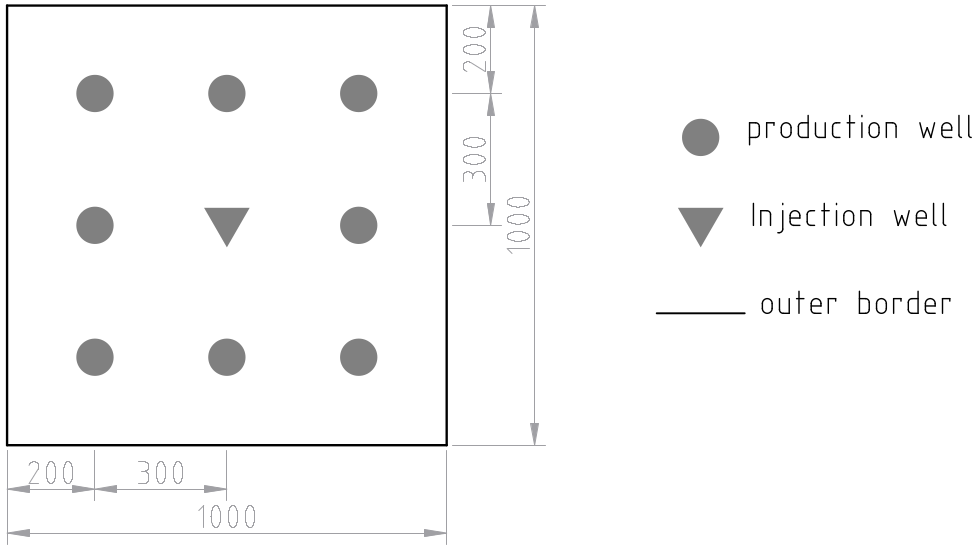
\includegraphics[height=6pc]{fig1.png}}
\begin{figure}
    \begin{minipage}[h]{0.69\linewidth}
      \center{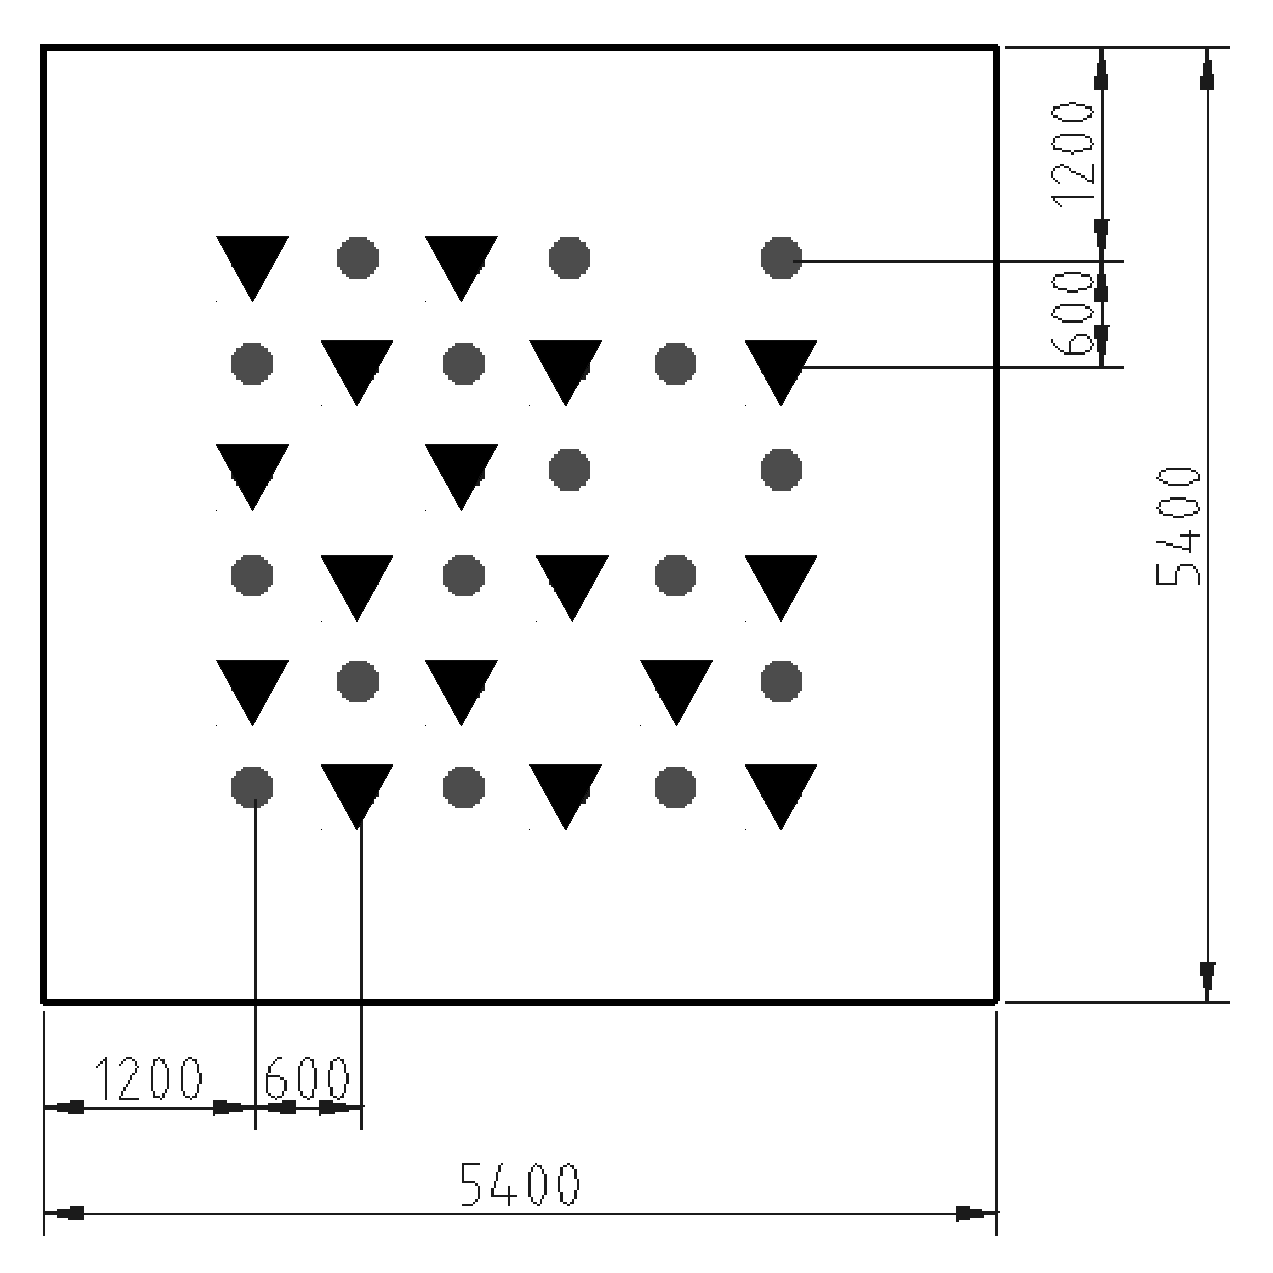
\includegraphics[width=20pc]{fig1a.eps}}
    \end{minipage} \hfill
    \begin{minipage}[h]{0.29\linewidth}
      \center{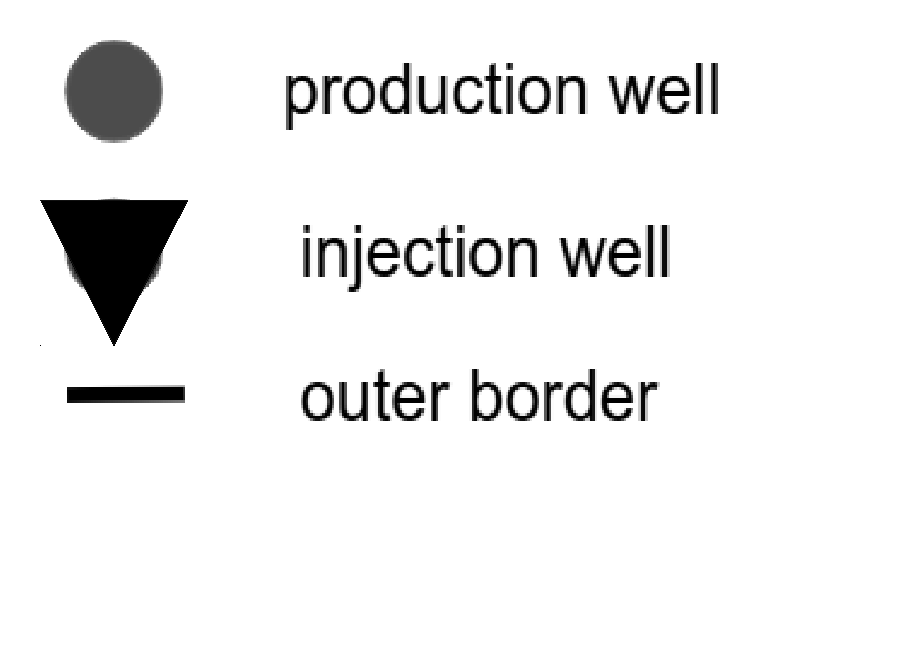
\includegraphics[width=6pc]{fig1b.eps}}
    \end{minipage} 
    \caption{Схематическое представление расчётной области.}
    \label{fig:map}
\end{figure}
Месторождение разрабатывается при помощи 16 добывающих и 16 нагнетательных скважин. Период разработки составляет 10 лет, контур питания был “подключён” по периметру расчетной области. Для решения задачи структурно-парамтерической идентификации период разработки был разбит на 3 интервала: 72, 24 и 24 месяца, соответсвенно:
\begin{enumerate}
\item с 01-2000 по 12-2005  интервал адаптации;
\item с 01-2006 по 12-2007  интервал валидации;
\item с 01-2008 по 12-2009  интервал прогноза.
\end{enumerate}

На интервале адаптации решается обратная задача для всех 4-х моделей, находятся неизвестные параметры. На интервале валидации оцениваются прогнозные характеристики настроенной модели, и осуществляется выбор модели, обладающей наилучшими прогнозными характеристиками. Дополнительно был выделен 3-й интервал - интервал прогноза, на котором производится оценка поведения выбраной модели при значительном изменении управляющих параметров. Временной интервал для этапа адаптации выбирался таким образом, чтобы он включал в себя поэтапный ввод в эксплуотацию всех скважин и был достигнут стационарный режим эксплуотации. Этап валидации включает в себя период стационарной работы месторождения. 

Для этапа прогнозирования было рассчитано 3 сценария эксплуатации для каждой модели, и произведено сопоставление поведение основных параметров разработки. В качестве сценариев были расчитаны: S0 - стационарный режим работы при котором не меняется объём нагнетаемой жидкости, S1 - двукратное сокращение объёма нагнетаемой жидкости и S2 - двукратное увеличение объёма нагнетаемой жидкости по сравнению со сценарием S0. 

На рисунке \ref{fig:din} представлена динамика среднего пластового давления для фактических данных (B - базовый вариант) и моделей водоносного горизонта (M1-M4 модели аквифера). На рисунке \ref{fig:hist} ввиде гистограммы показанны значения целевой функции (\ref{mape}) для интервалов адаптации (adp) и валидации (val), которая характеризует отличие вариантов M1-M4 от варианта B.
\begin{figure} 
    \begin{minipage}[h]{0.48\linewidth}
      \center{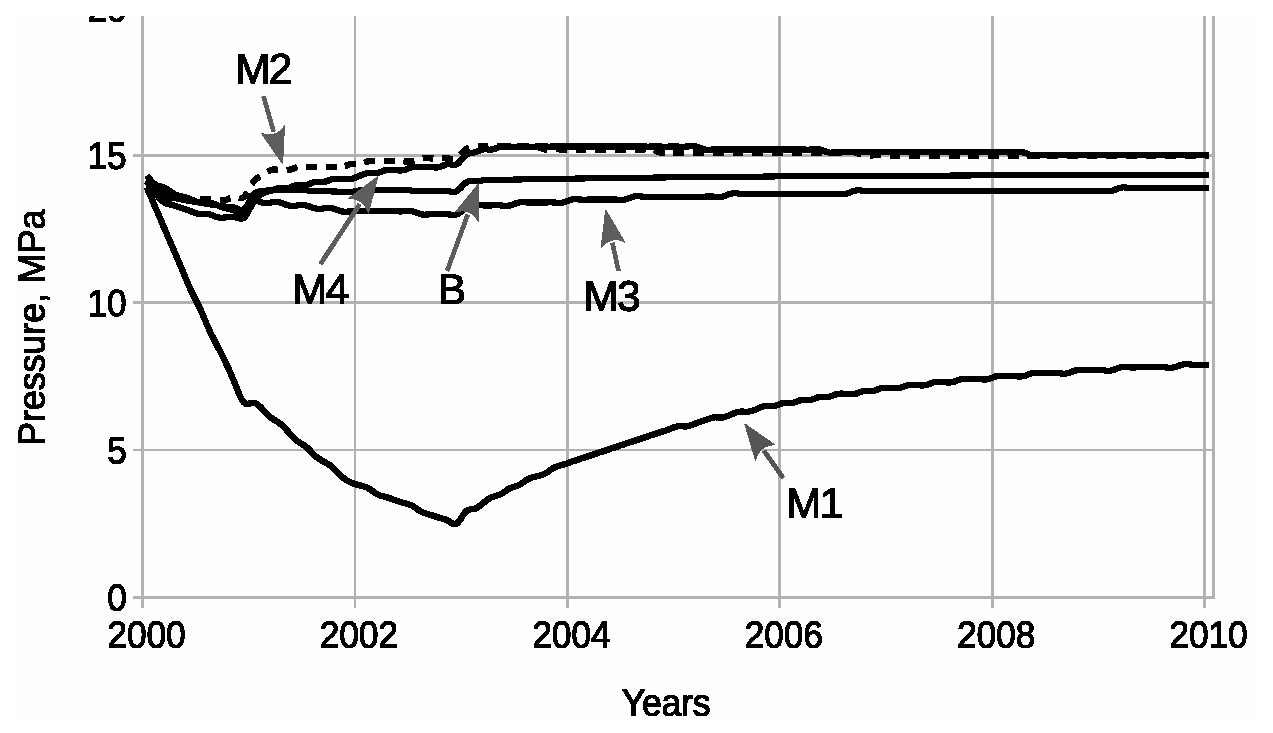
\includegraphics[height=0.60\linewidth]{fig2.eps}}
      \caption{Динамика среднего пластового давления при разных моделях водоносного горизонта}
      \label{fig:din}
    \end{minipage} \hfill
    \begin{minipage}[h]{0.48\linewidth}
      \center{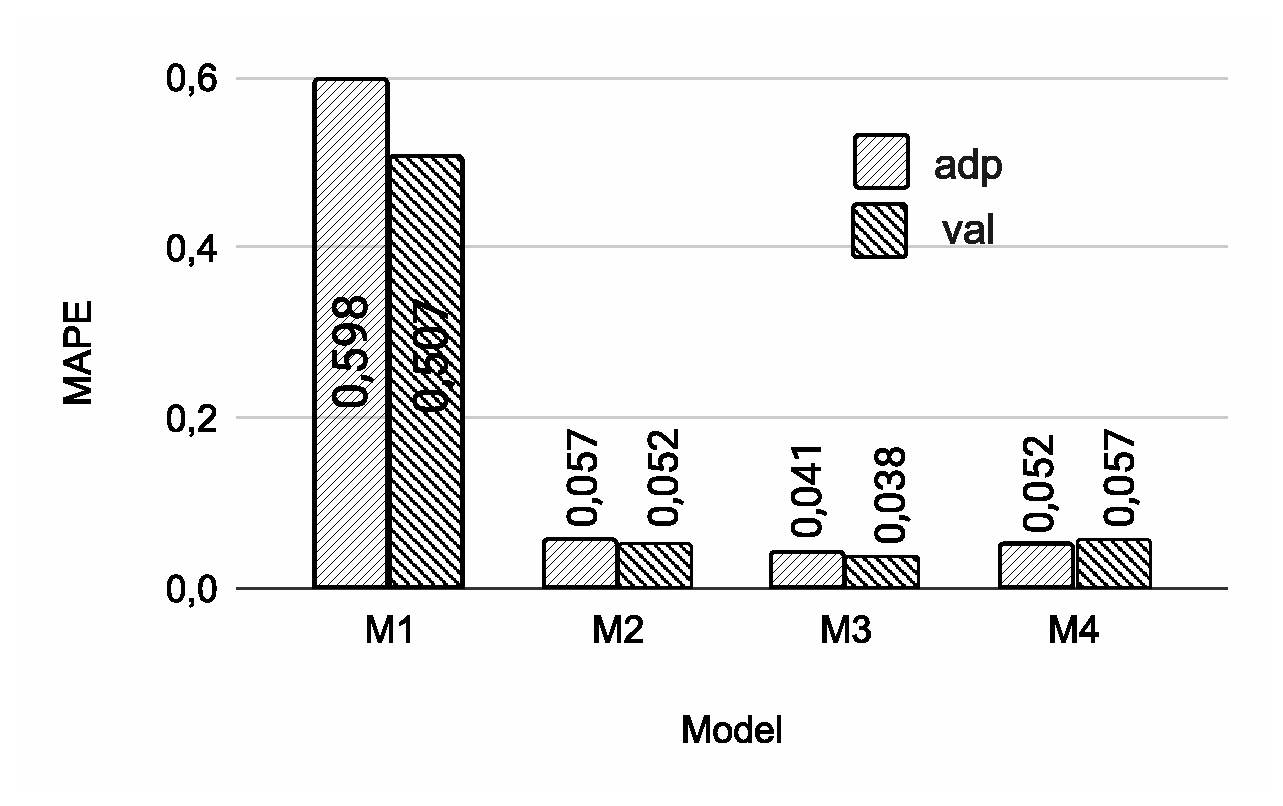
\includegraphics[height=0.60\linewidth]{fig3.eps}}
      \caption{Значения целевой функции для этапов адаптации (adp) и валидации (val)}
      \label{fig:hist}
    \end{minipage} 
\end{figure}
Из рисунков видно, что модель M1 обладает наихудшими показателями как на этапе адаптации так и на этапе валидации. Значение целевой функции примерно на порядок больше, чем у остальных моделей, следовательно, модель М1 наименне пригодня для описания поведения моделируемого объета и в дальнейших исследованиях она использоваться не будет. Наилучшими характеристиками для адаптации и валидации обладает модель M3. Модели M2 и M4 имею удовлетворительные значения целевой функции. Если сравнивать только две эти модели, то M4 лучше описывает историю, а M2 - имеет лучшие прогнозные свойства, соответсвенно выбор из этих двух моделей необходимо осуществлять используюя некоторые другие критерии например такие как BIC (\cite{mus}).

На практие, как правило, решеется только задача адаптации, и выбор модели осуществляется экспертно. Отбраковка моделей производится в основном по критерию не привышения ошибки, заложенной в различных регламентах (обычно от 5 до 25\%). Соотсветсвенно модели M2-M4 ввиду сравнительно малого отличия их показателей могут быть равновероятно выбраны в качестве прогнозирующих моделей. Действительно, наиболее ярко отличие динамики давления для разных моделей наблюдается в начальный период - при вводе новых скважин и выходе на стационарные режимы работы скважин. При стационарных режимах модели имеют близкие прогнозные характеристики. 

Интересным является поведение адаптированной модели при значительном (экстремальном) изменении режима работы скважин, реализованы в сценариях S1 и S2. На рисунке \ref{fig:2din} представлена динамика среднего пластового давления для трёх моделей (M2-M4) при трёх сценариях разработки (S0-S2).
\begin{figure}
\center{ 
    \begin{minipage}[h]{0.32\linewidth}
      \center{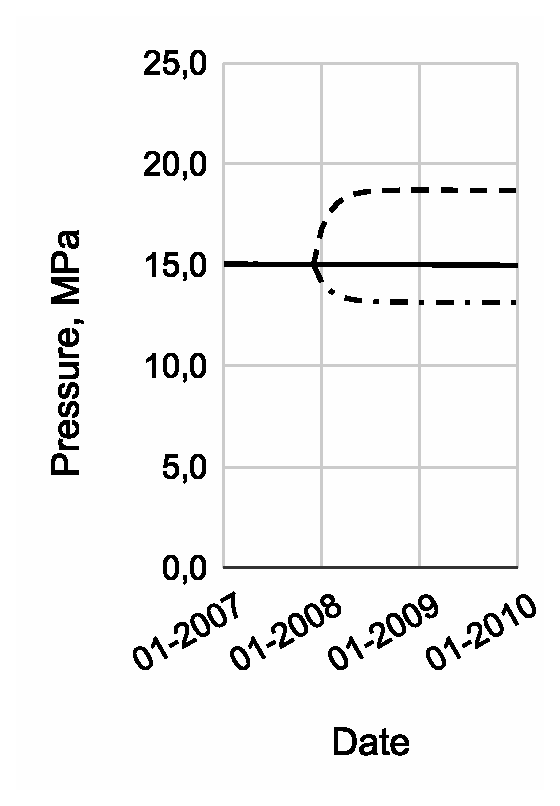
\includegraphics[height=0.92\linewidth]{fig4a.eps} \\ (a)}
    \end{minipage} \hspace{0pt}
    \begin{minipage}[h]{0.32\linewidth}
      \center{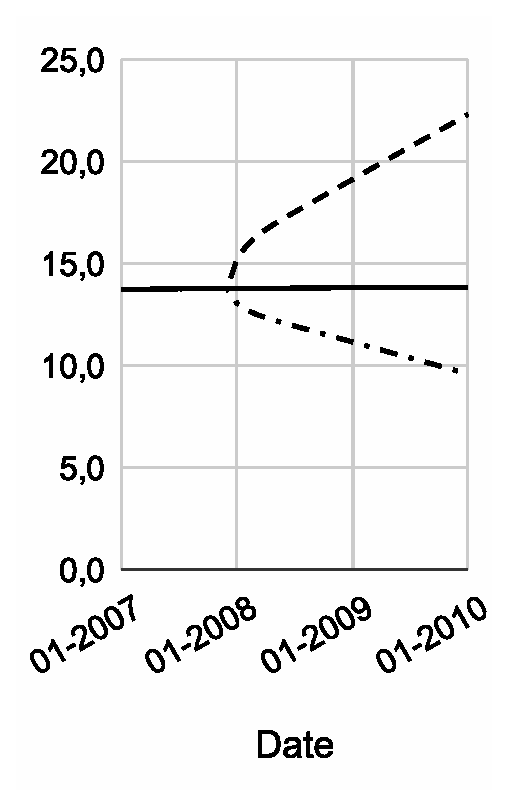
\includegraphics[height=0.92\linewidth]{fig4b.eps} \\ (b)}
    \end{minipage} \hspace{0pt}
    \begin{minipage}[h]{0.32\linewidth}
      \center{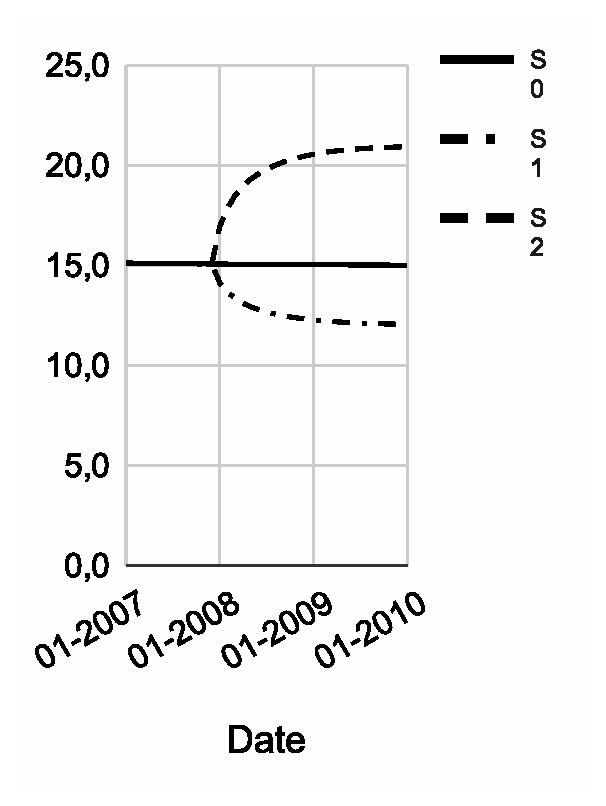
\includegraphics[height=0.92\linewidth]{fig4c.eps} \\ (c)}
    \end{minipage} 
    \caption{Динамика среднего пластового давления для 3-х моделей водоносного горизонта при 3-х сценариях разработки, где a, b и c соответствуют M2, M3 и M4.}
    \label{fig:2din}
    }
\end{figure}
Как видно из графиков, поведение кривых давления при одинаковых сценариях (S1 и S2) для разных моделей различны. Отличие заключается не только в значениях пластового давления, но и в динамике его изменения. Соответственно прогнозные показатели каждой модели будут существенно отличаться. Для поддержания качетва прогнозных свойств модели в допустимых пределах в условиях существенных изменений режимов работы, процедура актуализации модели является необходимой.

\section{CONCLUSIONS}

В результате исследования было показано, что получить удовлетворительное решение обратной задачи можно используя модели различной степени сложности. Помимо качества настройки модели на историю разработки - качества адаптации, также необходимо оценивать её прогнозные свойства. Проведение процедуры валидации позволяет осуществить выбор модели, имеющей наилучшие прогнозные характеристики. Кроме того, в работе было продемонстрированно, что качество прогноза помимо, сложности модели, зависит от сценариев разработки на которых адаптировалась и валидировалась модель. При  значительном отличии прогнозируемых режимов от тех, на которых была осуществлена настройка модели, прогнозные свойства модели резко снижаются. По мере поступления фактических данных необходимо заново проводить процедуру структурно-параметрической идентификации.

\section{FUNDING}
The research was carried out within the framework of the Program of Fundamental Scientific Research of the state academies of sciences in 2013-2020 (project No. AAAA-A17-117030610130-1).

%
% The Bibliography
%
\begin{thebibliography}{99}
\bibitem{mus} E.N.Musakaev, S.P.Rodionov, D.Y.Legostaev, V.P.Kosyakov,  «Parameter identification for sector filtration model of an oil reservoir with complex structure» // AIP Conference Proceedings 2125,030113 2019;

\bibitem{kos} V.P.Kosyakov, D.Y.Legostaev,  «Computational technology for solution of the reverse problem of filtration theory for oil fields with an aquifer» // AIP Conference Proceedings 2125,030112 2019;

\bibitem{bas} К.С.Басниев, Н.М.Дмитриев, Р.Д.Каневская, В.М.Максимов. Подземная гидромеханика.  М.-Ижевск: Институт компьютерных исследований, 2006. 

\bibitem{dake} L.P.Dake, Fundamentals of Reservoir Engineering (Elsevier, Amsterdam, 1978).

\bibitem{fet} M.J.Fetkovich. A Simplifi ed approach to water infl ux calculations – Finite aquifer systems. J. Pet. Tech. July 1971, vol. 23, is. 7, pp. 814–828.

\bibitem{opt} V.P.Kosyakov, S.P.Rodionov "Optimal control of wells on the basis of two-phase filtration equations". Proceedings of MIPT. 2016. V. 8, N 3. P. 79–90.


\end{thebibliography}

\end{document}